\chapter{3D Phase Tracking Monte Carlo Algorithm}\label{sec:phase}

\section{Introduction}\label{sec:besintro}

%Intro = mention complex beams and their uses then move onto gaussian and bessel beams



Bessel beams have been the subject of intense research since their discovery in 1987~\cite{durnin1987diffraction,durnin1987exact}. Durnin noticed that the blah blah.
%Bessel beams have since been used for blah blah
%They are really good and like are better than Gaussian beams allegedly.

This chapter examines how Bessel beams compare to other beam in a scattering medium. 
We investigate if the Bessel beams self-healing property has any effect in a turbid medium.
We examine Bessel beams and the other beams by creating a novel~\gls*{mcrt} algorithm that allows the tracking of a photon as it propagates through a medium. 
The main focus of this chapter, is validation of our new novel technique, followed by using the new algorithm ($\varphi MC$) to compare Gaussian and Bessel beams, to see which one preforms better in a turbid medium. 
This chapter also extends out novel algorithm to other complex, diffraction less beams


%motivation = better imaging of chick embryos etc


\section{Theory}\label{sec:bestheory}

The \gls*{mcrt} algorithm as described in~\cref{sec:mcrt}, must be adjusted so that wave phenomena such as interference and diffraction can be modelled. 
Modelling these wave behaviours allows us to model complex beams, where these phenomena are required to form the beam, e.g Bessel beams. 
As \gls*{mcrt} is a ballistic simulation of photon packets, meaning that the \gls*{mcrt} simulation presented thus far in this thesis only modelled the ballistic behaviour of photons. 
However for the work presented in this chapter, wave like behaviour is crucial to modelling the various experiments and phenomena.

To convert a ballistic simulation of photon packets into a ballistic/wave-like simulation, the complex phase of each photon packet is tracked.
This is achieved, by simply tracking the complex phase of the photon as it propagates through a medium.
~\Cref{eqn:phase} shows how the phase is calculated.

\begin{equation}
    \varphi = cos\left(\frac{2 \pi l}{\lambda}\right) + i\ sin\left(\frac{2 \pi l}{\lambda}\right)
    \label{eqn:phase}
\end{equation}

Where $\varphi~[-]$ is the phase of a photon packet, $l\ [m]$ is the distance the photons has travelled, $\lambda~[m]$ is the wavelength of the photon, and \textit{i} is the solution to $x^2=-1$.
Now we can calculate the phase of a photon at a position $P_o$, if we know the distance it has travelled, and its original phase,~\cref{fig:phase-diag}.

\begin{figure}[!ht]
    \centering
    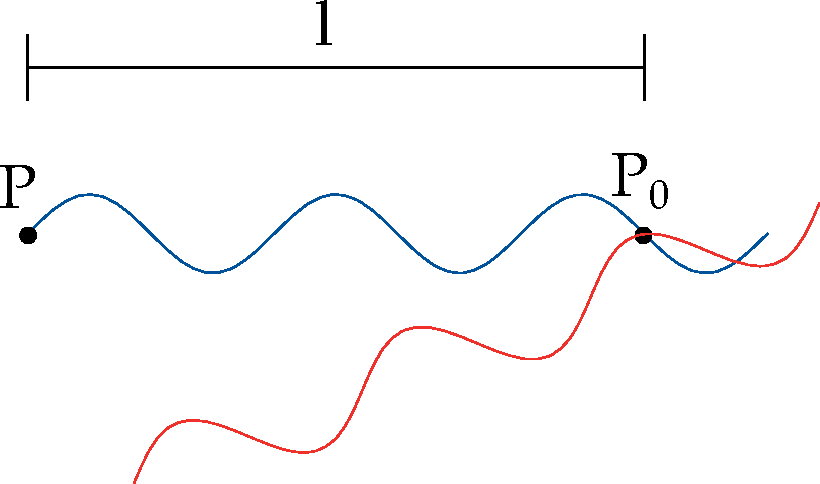
\includegraphics[width=0.5\textwidth]{phase-diag.pdf}
    \caption{Example of phase calculation when a photon has travelled a distance l. Figure also show an example of interference between two photons via addition of the complex amplitudes at the point $P_0$.}
    \label{fig:phase-diag}
\end{figure}

To be able model the wave-like behaviour of photons, we let the photons packets interfere with one another in a volume or area element. 
We do not model the interference at a point in space where photons packets cross one another as due to the ballistic nature of the \gls*{mcrt} simulation, this does not occur with enough frequency in order to give a good signal to noise ratio. 
Thus, interference takes place in a volume, $dV$, or area element, $dA$, instead.
To calculate the interference from the phase, the phase is summed in each volume or area element and the absolute value taken, and then squared.~\Cref{eqn:intense} shows the equation for interference for a volume element $dV$. A similar relation for calculating the interference on an area element $dA$ also exists.

\begin{equation}
I(\xi)=\left| \sum\limits_{\xi}cos\left(\frac{2\pi l}{\lambda}\right) + i \sum\limits_{\xi}sin\left(\frac{2\pi l}{\lambda}\right)\right|^2,\ \ \ \xi=(x,y,z)
\label{eqn:intense}
\end{equation}

\noindent Where:

\indent $l$ is the total distance travelled by a photon [$m$];

\indent $\lambda$ is the wavelength of the photon [$m$];

\indent $I$ is the intensity at the $\xi^{th}$ cell [$W m^{-2}$];

\indent and $\xi$ is the $x^{th}$, $y^{th}$, $z^{th}$ cell, volume $dV$.

\medskip

As the \gls*{mcrt} simulation is now a quasi ballistic/wave simulation of photon behaviour, comparisons between the simulations and, theoretical and experimental data to prove this model is accurate. However before validation of the model takes place, one further principle needs to be introduced that is required for our model to work.

\subsection{Huygens-Fresnel Principle}

The Huygens-Fresnel principle is a method that is used to help model the propagation of waves in the far field limit and the near field limit. 

The Huygens principle states~\cite{huygens2012treatise,hecht2017optics,huygens1900wave}: 

\medskip

``Every point on a propagating wavefront serves as the source of spherical secondary wavelets, such as the source at some time later is the envelope of these wavelets.''

\medskip

The principle is illustrated in~\cref{fig:huygensillis}. Christiaan Huygens postulated this principle in 1678.
The principle allowed Huygens to derive laws of refraction and reflection, but it failed to describe diffraction effects.
This led to Augustin-Jean Fresnel in 1818, combining the Huygens principle with his own theory of interference~\cite{fresnel1819memoire,huygens1900wave}.
This principle, the Huygens-Fresnel principle, gave an accurate description of the propagation of light and diffraction effects.
This was achieved by allowing the secondary wavelets to self interfere with one another, giving rise to an accurate description of the physical phenomena.
Later, Gustav Kirchhoff gave a rigours mathematical description of the Huygens-Fresnel principle, which is the basis of diffraction theory~\cite{kirchhoff1883ann,born2000principles}. 

The Huygens-Fresnel principle allows the modelling of diffraction in both the near and far field.
As the principle states that every point on the wavefront is a source of secondary spherical waves, this implies that there are ``backward'' waves.
These ``backward'' waves are unphysical, and there is no evidence of their existence.
Thus Fresnel introduced and inclination factor to eliminate these ``backward'' waves.
This inclination factor was later put on rigorous mathematical standing by Kirchoff, as it naturally fell out of his theory.~\cite{kirchhoff1883ann,born2000principles}

\medskip

Our algorithm uses the Huygens-Fresnel principle to simulate diffraction effects, that would otherwise be absent from the simulation.
The principle allows the algorithm to calculate the complex amplitude at a point, and thus the intensity at that point.
The Huygens-Fresnel principle is implemented by sampling the light source on the surface of any lens or in a slit.
In practise this means when for example, a plane wave is incident on a slit width \textit{a}, and length \textit{b}, the slit area is uniformly sampled for the initial position of the photon packets.
The packets are then given a random direction, sampled towards the detector thus avoiding the non-existent ``backward'' waves.
For the case of modelling propagation through a lens, the usual geometric optics approach is taken to propagate the packets through the lens.
When the packet lies on the surface of the lens, the Huygens-Fresnel principle is invoked, and the packet is given a random direction (in the direction of the medium) and propagated as usual.


\begin{equation}
u(\mathbf{r_1})=\frac{1}{i\lambda}\int\int u(\mathbf{r_0})\frac{\mathbf{\hat{s_0}} \cdot (\mathbf{r_1} - \mathbf{r_0})}{\left|\mathbf{r_1} - \mathbf{r_0}\right|^2}e^{ik\left|\mathbf{r_1} - \mathbf{r_0}\right|}dS_0
\end{equation}

\noindent Where:

    \indent $u$ is the complex electric field [$Vm^{-1}$];

    \indent $\lambda$ is the wavelength [$m$];

    \indent $S_0$ is a plane with surface normal $\mathbf{\hat{s_0}}$ [-];

    \indent $k$ is the wavenumber [$m^{-1}$];

    \indent and $r_n$ are spatial coordinates [-].

\medskip

This is the principle that underpins the algorithm that allows various complex beams, and wave phenomena to be simulated within a ballistic method. The following sections validate the method against the theory and experimental data for various complex beam propagation.

\begin{figure}[!ht]
    \centering
    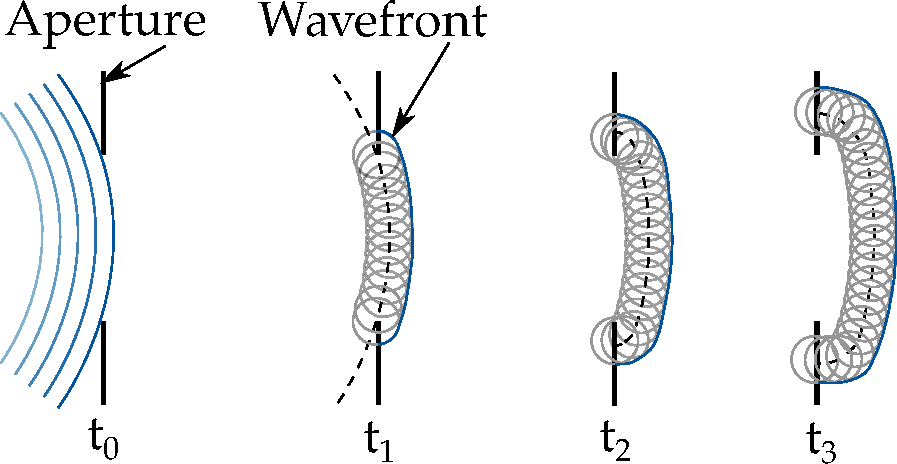
\includegraphics[width=0.7\textwidth]{huygens.pdf}
    \caption{Illustration of the Huygens-Fresnel principle. At $t_0$ a wave is incident on an aperture. Times $t_1,\ t_2,\ \text{and}\ t_3$ show the evolution of the wavefront using the Huygens-Fresnel principle.}
    \label{fig:huygensillis}
\end{figure}

\subsection{Validation of Phase Tracking Algorithm}

\subsubsection*{Double Slit Experiment}

The first test of our phase tracking algorithm, is to compare our simulation to a double slit experiment.
The double slit experiment, is a simple experiment where monochromatic plane wave of light is incidence on two slits distance apart $a$, and width $b$, and the interference pattern is observed on a screen a distance $d$ away from the slits.

This experiment, first carried out by Thomas Young and thus sometimes called Young's slits experiment, is usually carried out with the detector screen in the far field. The so called Fraunhofer regime.
The intensity pattern on the detector screen is as in\cref{eqn:doubleslit}:

\begin{equation}
    I(\theta) \propto cos^2\left(\frac{\pi d\ sin \theta}{\lambda}\right)sinc^2\left(\frac{\pi b\ sin\theta}{\lambda}\right)
    \label{eqn:doubleslit}
\end{equation}

Where the $sinc$ function is defined as $\tfrac{sin(x)}{x}$, for $x\ \neq 0$, d is the slit separation and $\theta$ is the angular spacing of the fringes.

The simulation was carried out for a wavelength of , a slit width of, and a slit separation of .
Using the Huygens-Fresnel principle, each slit is a source of Huygens wavelets.
The initial position of the photon packets is sampled uniformly from the slit area, after randomly choosing one of the slits.
A random direction is then chosen to ensure that the packets will hit the detector screen.
The simulation was run with photon packets, which took to run on an 8 core Intel Xeon machine.
This gave an accurate match to the theoretical expression, as seen in~\cref{fig:doubleslitcomp}.


\begin{figure}[!ht]
    \centering
    % \includegraphics[]{}
    \caption{Comparison of theory and simulation for the double slit experiment. $\lambda$ is $x nm$, $b$ is, and $d$}
    \label{fig:doubleslitcomp}
\end{figure}

\subsubsection*{Diffraction by a Square Slit}
$\varphi MC$ is also validated by simulating diffraction from a square aperture in the far and near field, the so call Fresnel and Fraunhofer regimes. 
Fresnel diffraction occurs in the near field when the \textit{Fresnel number},~\cref{eqn:fnumber}, is greater than 1.0.
Fraunhofer diffraction occurs when the \textit{Fresnel number} is less than 1.0.

\begin{equation}
F = l\sqrt{\frac{2}{\lambda r_0}}
\label{eqn:fnumber}
\end{equation}

\Cref{eqn:fnumber} is the Fresnel number, a measure of whether diffraction is in the Fresnel regime or the Fraunhofer regime.
\textit{l} is the slit width, $\lambda$ is the wavelength of the incident radiation, and $r_0$ is the distance from the aperture to the detector screen, as shown in~\cref{fig:aperture}. 

\medskip
\begin{figure}[!ht]
    \centering
    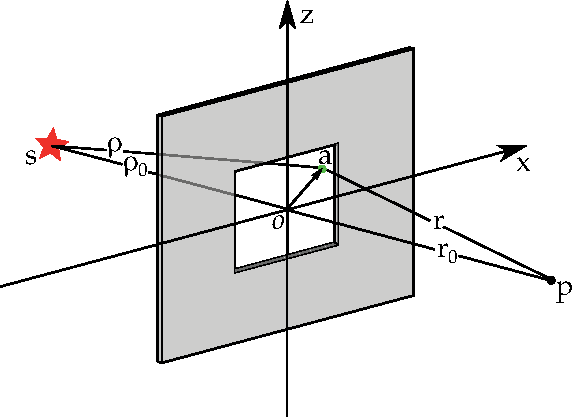
\includegraphics[width=0.75\textwidth]{aperture.pdf}
    \caption{Fresnel diffraction at a square aperture.}
    \label{fig:aperture}
\end{figure}

In order to compare $\varphi MC$ to the theory, the theory must first be examined.
Consider the setup as shown in~\cref{fig:aperture}, in order to calculate the intensity at a point $P$, the contribution by an area element $dS$ at the point a, to the optical disturbance at a point \textit{P} is considered.
Accounting for the the unobstructed optical disturbance from $S$ as well, yields: 


\begin{equation}
U(P)=\frac{1}{i\lambda}\iint\limits_{\Sigma} \frac{Ae^{i(k\rho-\omega t)}}{\rho} \frac{e^{ikr}}{r}cos(\theta)\ dS
\label{eqn:disturb}
\end{equation}


In the case where $\rho_0$ and $r_0$ are large compared to the size of the aperture, then $cos(\theta) = 1$ and $\tfrac{1}{\rho r}=\tfrac{1}{\rho_0 r_0}$.
The lengths of $r_0$ and $\rho_0$ are:

\begin{align}
r=&\sqrt{r_0^2+y^2+z^2}\label{eqn:r} \\
\rho=&\sqrt{\rho_0^2+y^2+z^2}\label{eqn:rho}
\end{align}

Using the binomial theorem to expand~\cref{eqn:r,eqn:rho} yields:

\begin{equation}
\rho + r \approx \rho_0 + r_0 + (y^2+z^2)\frac{\rho_0r_0}{2\rho_0r_0}
\label{eqn:binomial}
\end{equation}

Substituting~\cref{eqn:binomial} into~\cref{eqn:disturb} with $k=2\pi/\lambda$

\begin{equation}
U(P)=\frac{Ae^{-i[k(\rho_0+r_0)\omega t]}}{i\lambda\rho_0r_0}\iint\limits_{\Sigma} e^{i2\pi y^2\tfrac{(\rho_0+r_0)}{2\lambda\rho_0r_0}+i2\pi z^2e^{\frac{i\pi u^2}{2}}\tfrac{(\rho_0+r_0)}{2\lambda\rho_0r_0}} \ dS
\label{eqn:midway}
\end{equation}


Introducing the dimensionless variables \textit{u} and \textit{v}

\begin{align}
u&=y\sqrt{\frac{2(\rho_0+r_0)}{\lambda\rho_0r_0}}\\
v&=z\sqrt{\frac{2(\rho_0+r_0)}{\lambda\rho_0r_0}}
\end{align}

and substituting them into~\cref{eqn:midway}.

\begin{equation}
U(P)=\frac{\tilde{E}_u}{2}\int_{u_1}^{u_2} e^{\tfrac{i\pi u^2}{2}}\ du\int_{v_1}^{v_2} e^{\tfrac{i\pi v^2}{2}} \ dv
\label{eqn:pentdisturb}
\end{equation}
\Cref{eqn:pentdisturb} describes the optical disturbance at the point $P$, with $\tilde{E}_u$ the unobstructed disturbance at $P$.
\Cref{eqn:pentdisturb} can be evaluated using the Fresnel integrals, $C(w)$ and $S(w)$:


\begin{equation}
\int_{0}^{w}e^{i\pi w'^2/2}dw'=C(w)+iS(w)
\label{eqn:fresneleqn}
\end{equation}


\begin{align}
S(w)&=\int^w_0 sin\left(\frac{\pi w'^2}{2}\right)dw'\label{eqn:fresint1}\\
C(w)&=\int^w_0 cos\left(\frac{\pi w'^2}{2}\right)dw'\label{eqn:fresint2}
\end{align}


Using~\cref{eqn:fresneleqn}, where $C(w)$ and $S(w)$ are the Fresnel integrals as in~\cref{eqn:fresint1,eqn:fresint2},~\cref{eqn:pentdisturb} can then be transformed into an intensity, by taking the absolute value and squaring, yielding~\cref{eqn:fresIntensityp}:


\begin{equation}
I_p = \frac{I_u}{4} \{[C(u_2) - C(u1)]^2 + [S(u_2) - S(u_1)]^2\} \times \{[C(v_2) - C(v_1)]^2 + [S(v_2) - S(v_1)]^2\}
\label{eqn:fresIntensityp}
\end{equation}

\Cref{eqn:fresIntensityp} gives the intensity of the field at the point $P$ on axis for a square aperture where $I_u$ is the unobstructed intensity at the point $P$. 

\medskip

As the mathematics of calculating the optical disturbances at all points on a plane at point $P$ is difficult, instead the aperture is moved by small displacements, with $\overrightarrow{SOP}$ fixed.
This effectively achieves the translation of the origin, $O$, with respect to the fixed aperture. 
Thus, for each displacement new aperture coordinates $y_1, y_2, z_1, \text{and } z_2$ are generated and therefore new $u_1, u_2, v_1, \text{and }v_2$.
Therefore the intensity at a point $P +\delta d$, where $\delta d$ is the displacement, can be calculated.
This approximation holds for displacements that are small compared to the $\rho_0$~\cite{born2000principles,hecht2017optics,goodman2017introduction}.
Using this method and~\cref{eqn:fresIntensityp} gives the theoretical curves curves in~\cref{fig:frescompare}.

\medskip

In $\varphi MC$, the above experiment is simulated. 
A square slit is uniformly sampled in the $y$, and $z$ direction in order to get the packets initial position. 
A random direction is then sampled, ensuring that the direction points towards the detector screen.

The detector screen's distance from the aperture is then varied and the intensity on the screen is measured for $\sim 10^{10}$ photons released from the aperture, as Huygens wavelets.
For \textit{Fresnel numbers} greater than 1.0, the number of bins is 300, covering a distance of 600~$\mu m$. 
For the case of Fraunhofer diffraction, the number of bins is 100 covering a distance of 6000~$\mu m$.
The simulations take $\sim$ 3 minutes for $10^{10}$ packets to be run on an Intel Xeon E3--1245 v5, 8 cores @ 3.5GHz machine.
The number of bins, and photons packets simulated had to be increased for the cases where the Fresnel number was large (i.e the detector screen was near the aperture)
\cref{fig:frescompare} shows the comparison between the theory and the $\varphi MC$ simulations.

\begin{figure}[!ht]
    \centering
    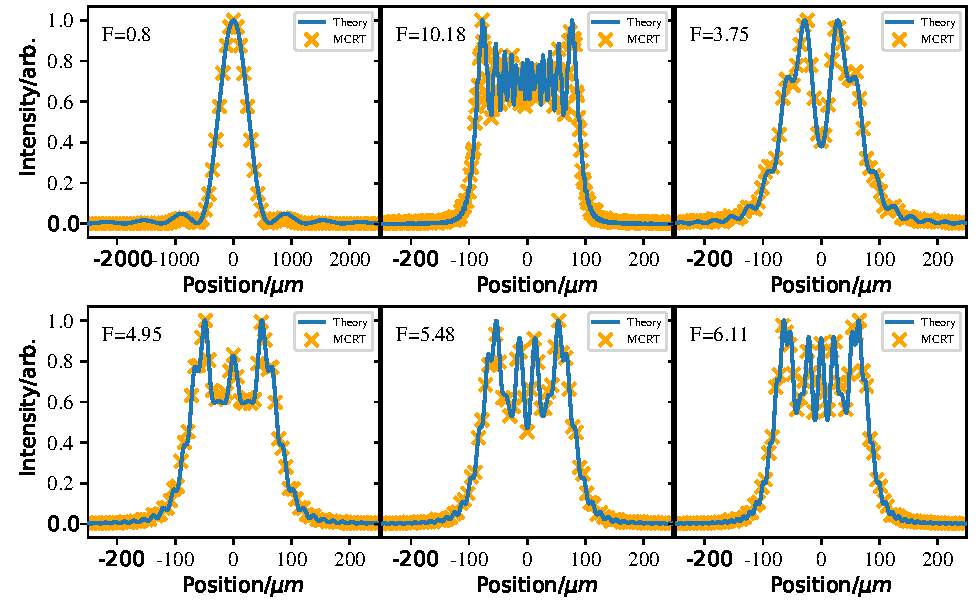
\includegraphics[width=0.75\textwidth]{Fresnel-compare.pdf}
    \caption{Comparison of theory and simulation for diffraction through a square aperture in the Fresnel and Fraunhofer regimes.}
    \label{fig:frescompare}
\end{figure}

\FloatBarrier

\section{Bessel Beams}

Bessel beams, as described in the introduction to this chapter, are ``non--diffracting'' beams, that can ``self heal''.
This means, in reality, that the central core of the beam does not spread out, and that if a blockage is placed in front of the beam, the beam reforms further down the optical axis.
There is some debate amongst physicists as to weather these phenomena are justly labelled, or if they glib terms used to make Bessel beams seem like the solution to everything.

The first ``complex'' beam simulated using $\varphi MC$ is a Bessel beam. 
Bessel beams are non-diffractive solutions to the wave equation. 
Bessel beams were first shown to blah


% *** Bessel beams non diffracting
%     but are they - some debate over this
%     self reconstructing
%     central core does not diffract like Gaussian
%     quasi Bessel beam -> infinite rings not possible -> infinite energy
%     Bessel beam theory form of equation -> intensity
%     pics of Bessel beam + higher orders
%     geometry of Bessel beams
%     Bessel beams in code
%     results
% ***

% *** add in general lth order eqn***
From the scalar description of the electric component of the beam, we get:

\begin{equation}
    E(r,z)=E_0\sqrt{\frac{2\pi k z w_0sin(\beta)}{z_{max}}}\ \text{exp}^{\left(-\frac{z^2}{z_{max}^2}-\frac{i\pi}{4}\right)}\ J_0\left(krsin(\beta)\right)\ \text{exp}^{\left(ikzcos(\beta)\right)}
    \label{eqn:besselEfield}
\end{equation}

\noindent Where:

    \indent k is the wavevector, $k=\tfrac{2\pi}{\lambda}$ [$m$];

    \indent z is the distance from the axicon tip [$m$]; 

    \indent $\beta$ is the angle the wavefront propagates at (see~\cref{fig:besselgeo}) [$rad$]; 

    \indent $w_0$ is the $\tfrac{1}{e^2}$ width of the input Gaussian beam [$m$]; 

    \indent $J_0$ is the Bessel function of the first order; 

    \indent r is radial distance from the optical axis [$m$]. 

\medskip


~\Cref{eqn:besselEfield} gives the electric field for a Bessel beam. The intensity can be calculated using:

\begin{equation}
    I(r,z)=\frac{c\epsilon_0\left|E\right|^2}{2}
    \label{eqn:besselintsub}
\end{equation}

Using the definition total power transmitted by a beam as:

\begin{equation}
    P=\frac{\pi I_0w_0^2}{2}
    \label{eqn:pwrdef}
\end{equation}

Where $I_0$ is defined as on axis intensity of the incident Gaussian beam.

\begin{equation}
    I_0=\frac{c\epsilon_0E_0^2}{2}
    \label{eqn:intdef}
\end{equation}

Substituting~\cref{eqn:besselEfield,eqn:intdef,eqn:pwrdef} into~\cref{eqn:besselintsub} yields:

\begin{equation}
    I(r,z)=\frac{4k_rP}{w_0}\frac{z}{z_{max}}J_0^2\left(k_r\ r\right)\text{exp}^{\left(-\frac{2z^2}{z^2_{max}}\right)}
    \label{eqn:besselInt}
\end{equation}


\noindent Where:

    \indent $k_r$ is the radial wavevector, $k_r=k\ sin(\beta)$;

    \indent P is the power of the incident Gaussian beam.

    \medskip

Bessel beam can be formed by an axicon lens or by diffraction through a ring.
All the simulations of Bessel beams in this thesis use the axicon method of generating a Bessel beam, thus only axicons will be discussed.
\Cref{fig:besselgeo} shows the geometry of a Bessel beam formed by an axicon.
Using simple geometry and Snell's law the following equation can be derived to describe various properties of a Bessel beam formed by an axicon~\cite{merola2012characterization,}.

The propagation depth of a Bessel beam is defined as the distance from the tip of the axicon to the end of the ``Bessel region''. However in reality the Bessel beam will continue to propagate slightly passed this depth.%***source
~\Cref{eqn:besselzmax} shows the propagation depth of a Bessel beam where $cot$ is the cotangent function.
\begin{equation}
z_{max}=R\left(cot\left(\beta\right) - tan\left(\alpha\right)\right)
\label{eqn:besselzmax}
\end{equation}

The propagation angle of the conical waves, $\beta$ can be calculated using Snell's law and $\alpha$ the angle of the axicon:

\begin{equation}
\beta = arcsin\left(n\ sin\left(\alpha\right)\right)-\alpha
\label{eqn:betaangle}
\end{equation}

The central core of a Bessel beam is defined as the distance to the first zero of the Bessel beam.
\Cref{eqn:coreradius} shows the radius of the core, where $2.405$ is derived from position of the first zero of the Bessel function.

\begin{equation}
r_o = \frac{2.405}{k\ sin\left(\beta\right)}
\label{eqn:coreradius}
\end{equation}

Finally, the spacing between Bessel beam rings is:
\begin{equation}
\Delta \rho = \frac{\lambda}{2\ sin\left(\beta\right)}
\end{equation}

\subsection{Validation}

To ensure that the method described in~\namecref{sec:bestheory} works as intended for Bessel beams several tests are run against theoretical expressions and experimental data.

\subsubsection*{Comparison to theoretical Bessel beam}

To compare against a theoretical Bessel beam, a Bessel beam is modelled in the~\gls*{mcrt} phase simulation, and propagated through air into the ``Bessel region'' and then propagated into the far field to ensure the beam follows the theory in both these regions.

\Cref{fig:besselgeo} shows the setup for the \textit{in-silico} experiments.
The Bessel beam is created with an axicon (conical) lens with an opening angle ($\alpha$) of $5^{\circ}$, and a radius of $12.7~mm$.
The input beam is Gaussian in profile with a $\tfrac{1}{e^2}$ diameter of $1~mm$, and a wavelength of $488~nm$.
The Bessel beam is then propagated to a detector screen $10~mm$ away from the tip of the axicon, which is in the middle of the ``Bessel region'' for the first test.
for the second test the Bessel beam is propagated past the ``Bessel region'' into the far field.
The detector screen has a size of $40~mu m$ $\times$ $40~mu m$ with a bin resolution of $1~\mu m$.
$8^10$ photon packets were simulated taking $\sim$ 1 hour on an 8 core Intel Xeon 3.5Ghz machine.

\medskip

~\Cref{eqn:besselInt} gives the profile of a theoretical Bessel beam at a depth $z_{max}$, this is plotted against the simulation when $\tfrac{4k_rPz}{w_0z_{max}}e^{-2\left(\tfrac{z}{z_{max}}\right)^2}=1$, with the simulation similarly normalised, by normalising to the maximum intensity of the image generated. ~\Cref{fig:besselCompare} shows this comparison.

\Cref{fig:farfield} shows the profile of the Bessel beam in the far field, where the theory predicts that it becomes a circular beam.

\begin{figure}[!ht]
    \centering
    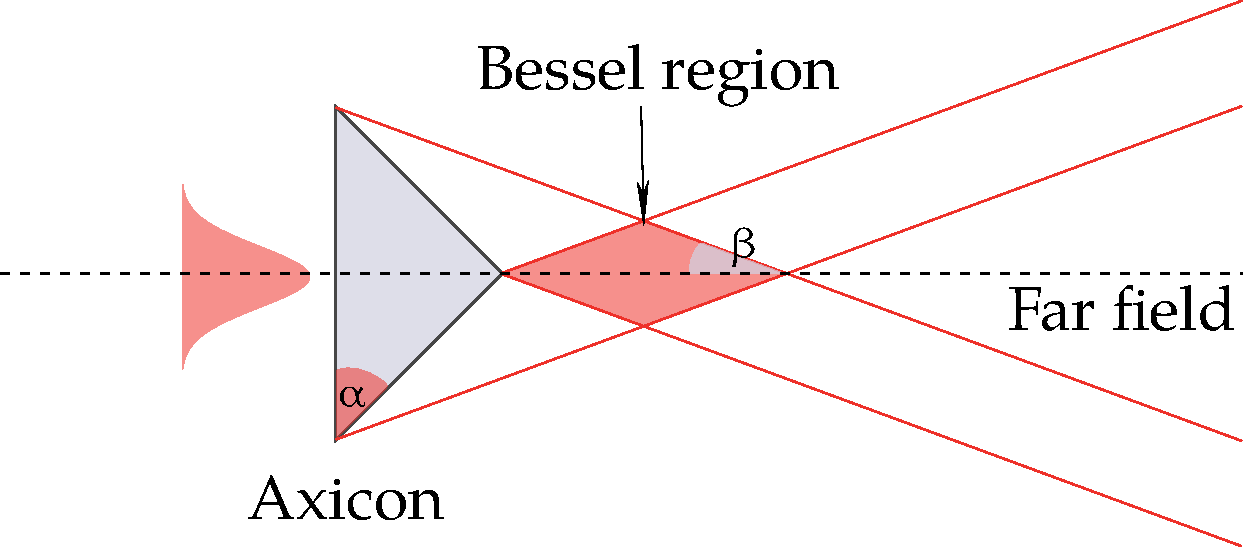
\includegraphics[width=0.6\textwidth]{bessel.pdf}
    \caption{Geometry of a Bessel beam, generated by an axicon lens. $\beta$ is the angle with the optical axis, and the angle of the conical waves. $\alpha$ is the axicon angle.}
    \label{fig:besselgeo}
\end{figure}




\begin{figure}[!ht]
    \centering
    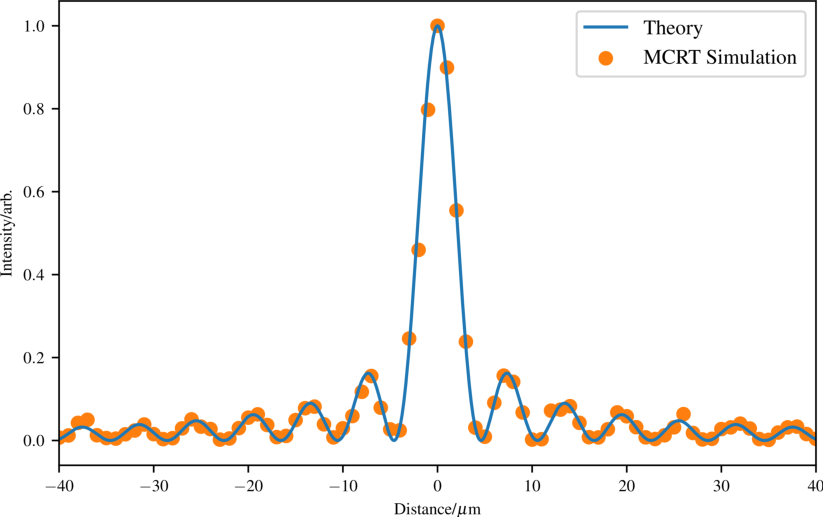
\includegraphics[width=0.75\textwidth]{compare-theory.pdf}
    \caption{Comparison of theoretical and MCRT simulation of a Bessel beams, with intensity normalised. The results from $\varphi MC$ show good agreement with the theory.}
    \label{fig:besselCompare}
\end{figure}

\begin{figure}
\centering
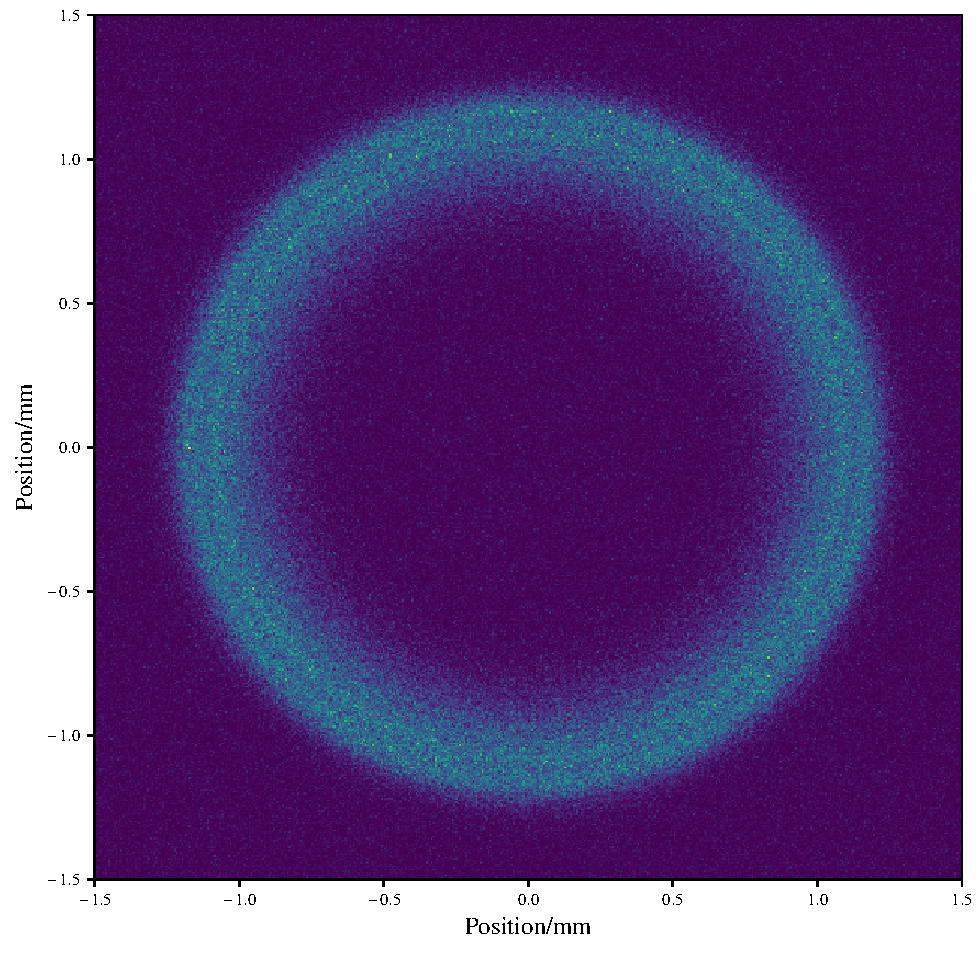
\includegraphics[width=0.75\textwidth]{farfield.pdf}
\caption{Bessel beam in the far field.}
\label{fig:farfield}
\end{figure}

\FloatBarrier

\subsubsection*{Comparison to experimental data}

To ensure our algorithm works in turbid media, we carried out an experiment where a Bessel beam was propagated through a medium of varying turbidity.
A laser, wavelength $488~nm$, with a Gaussian profile is shone on an axicon lens, with angle $5^{\circ}$.
The laser beam had a $\tfrac{1}{e^2}$ diameter of $2~mm$. 
The Bessel beam was allowed to propagate through the air for $10~cm$ before entering a cuvette of side $2~mm$.
The cuvette was filled with $500~\mu L$ of water, and various volumes of a scattering agent added.
The scattering agent used is intralipid $20~\%$ (Sigma-Aldrich), which is diluted as shown in~\cref{tab:intra}.
~\Cref{fig:ilscatprop} shows the optical propeties of Intralipid $20~\%$.
Dilutions of Intralipid are kept below 2\% scattering particle concentration, so that the scattering exhibited by the intralipid is in the independent scattering regime.
This allows the linear scaling of the optical properties by concentrations~\cite{aernouts2013supercontinuum,vardaki2015studying,di2011effect}.
Images of the Bessel beam as it emerges from the cuvette are taken for comparison with out algorithm.
~\Cref{fig:expsetup} shows the experimental setup.

\begin{figure}[ht!]
    \centering
    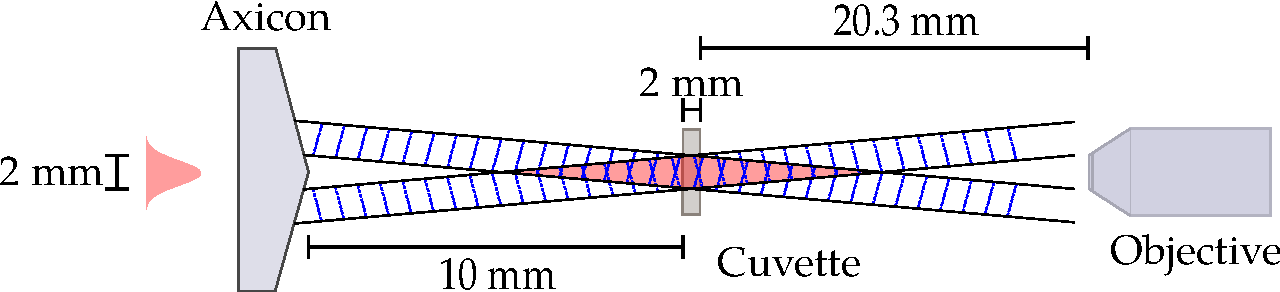
\includegraphics[width=0.8\textwidth]{bessel-exp-setup.pdf}
    \caption{Experimental setup for propagating a Bessel beam through a cuvette filled with varying concentrations of Intralipid 20\%. Bessel beam is imaged by an $20\times$ objective lens and a Grasshopper 3 camera.}
    \label{fig:expsetup}
\end{figure}


\begin{table}[!ht]
    \begin{tabular}{cc|cc|c}
        \hline
        \multicolumn{2}{c|}{Volume/$\mu L$} & \multicolumn{2}{c|}{Intralipid concentration}                       & Optical properties              \\
        Intralipid                & $H_2O$  & Volume/\%      & Scattering particle/\%                             & Scattering coefficient/$m^{-1}$ \\ \hline
        \multicolumn{1}{c|}{0}    & 500     & \multicolumn{1}{c|}{0.00}    & 0.00                                 & 0.00                            \\
        \multicolumn{1}{c|}{2}    & 500     & \multicolumn{1}{c|}{0.39841} & 0.0908                               & 557.14                          \\
        \multicolumn{1}{c|}{4}    & 500     & \multicolumn{1}{c|}{0.79365} & 0.1816                               & 1114.28                         \\
        \multicolumn{1}{c|}{6}    & 500     & \multicolumn{1}{c|}{1.18577} & 0.2724                               & 1671.42                         \\
        \multicolumn{1}{c|}{8}    & 500     & \multicolumn{1}{c|}{1.57480} & 0.3632                               & 2228.56                         \\
        \multicolumn{1}{c|}{10}   & 500     & \multicolumn{1}{c|}{1.96078} & 0.4534                               & 2785.71                         \\
        \multicolumn{1}{c|}{12}   & 500     & \multicolumn{1}{c|}{2.34375} & 0.5448                               & 3342.84                         \\ \hline
    \end{tabular}
    \caption{Intralipid solutions used for experiment.}
    \label{tab:intra}
\end{table}

\begin{figure}[!ht]
    \centering
    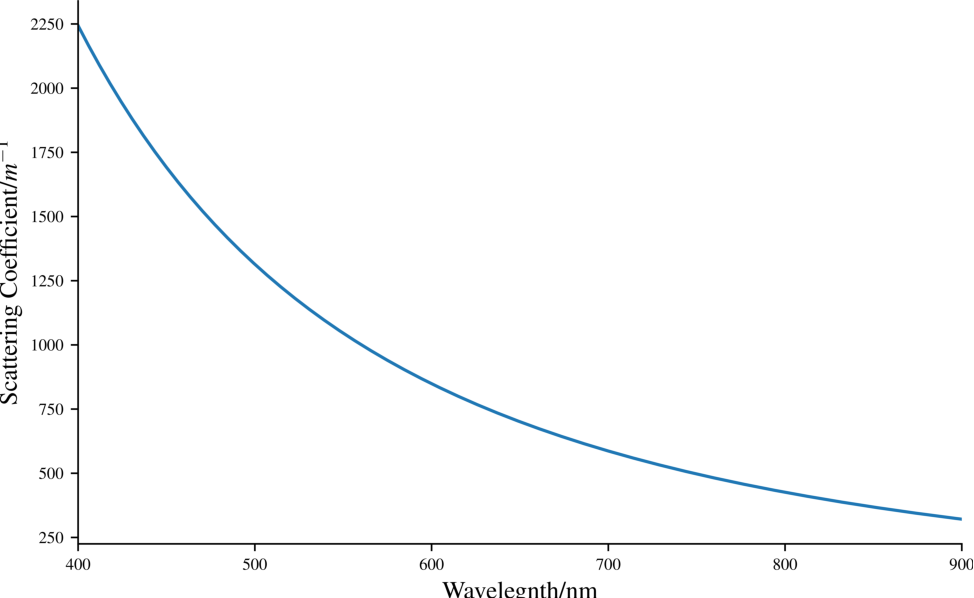
\includegraphics[width=0.7\textwidth]{scat-prop-il.pdf}
    \caption{Scattering properties of 20\% Intralipid~\cite{michels2008optical}.}
    \label{fig:ilscatprop}
    \vspace{-10pt}
\end{figure}

To model within $\varphi MC$, the experimental setup we simplify the setup considerably.
The simulation models the propagation of a photon packet through the axicon to its conical surface. 
On the conical surface the Huygens-Fresnel principle is invoked, and the packet is sampled onto the surface of the medium (cuvette).
The sampling of the photon onto the surface of the medium, speeds the algorithm up, as it does not need to simulate the photons that would ``miss'' the medium.
From there the usual~\gls*{mcrt} method propagates the packet through the medium while tracking its phase, and scattering the packet until it leaves the medium.
If the packet leaves the medium to any side other than the far side of the cuvette (e.g any side of the cuvette not facing the objective lens), then it is discarded.
If the packet leaves the medium on the objective lens facing side, then the packet is recorded by its phase onto an area element.
For each intralipid concentration $6.4\times10^{10}$ photons are run over 64 cores, taking $\sim 3$ hours for the 0.5448\% intralipid concentration.
Once all the photon packets have been run, the phase is converted into intensity, as in~\cref{eqn:intense}, but in 2D.

\Cref{fig:compareexpbessel} shows the results from the experiment and simulation. The simulation shows good agreement with experimental data.

\begin{figure}[!ht]
\centering
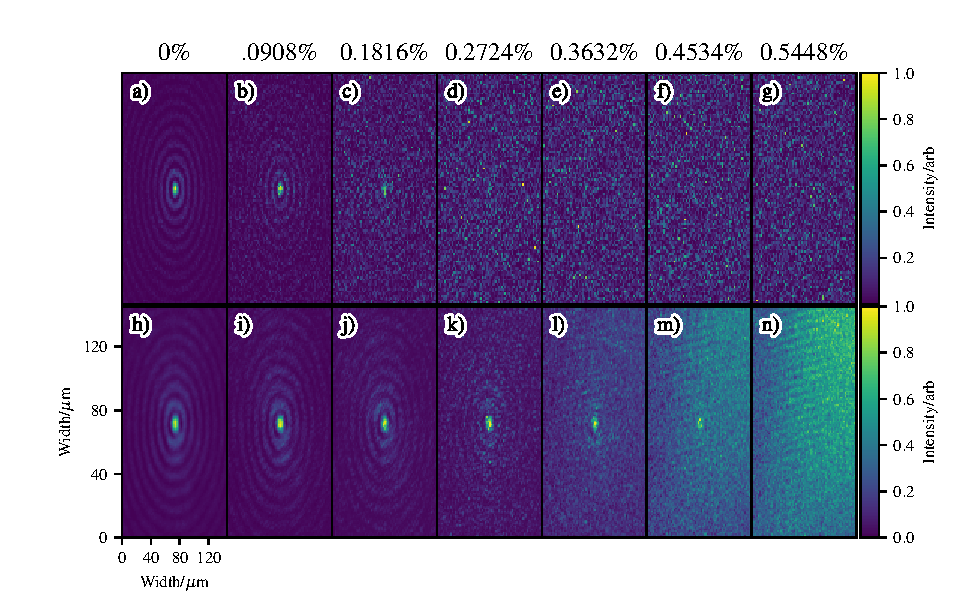
\includegraphics[width=0.95\textwidth]{compare-exp.pdf}
\caption{Comparison of experimental and simulation data for propagation of a Bessel beam produced by an axicon, through mediums of various turbidity. Images a) to g) is the data from $\varphi MC$, and h) to n) are the experimental data. Volumes along the top is the volume of Intralipid in each solution as in~\cref{tab:intra}. All images cropped so they are the same size.}
\label{fig:compareexpbessel}
\end{figure}

\subsubsection*{Discussion}

Originally the medium was modelled as in the experiment, a $2~mm^3$ volume.
The image created was thus a $2001 \times 2001$ with a resolution of $1~\mu m$.
In order to achieve a good signal to noise ratio for this setup $6.4\times10^{12}$ packets needed to be run, taking $\sim$ 70 hours on a computer cluster using 64 cores.
This was enough packets to get a good signal to noise ration on all the simulations up to $6~\mu L$.
However the amount of packets needed to get a good signal to noise ratio for $8~\mu L$ and above was prohibitively computationally costly.
Therefore the modelled medium was shrunk in the \textit{x} and \textit{y} directions giving: $0.5~mm \times 0.5~mm \times 2.0~mm$.
This allowed a smaller image (501 $\times$ 501), whilst keeping the same resolution.
Shrinking the medium also has the benefit that the photons are confined closer to the image plane, thus ensuring more photons are hit the plane in comparison to the larger medium. 

Shrinking the mediums size does have some draw backs.
Firstly Bessel beams propagation depth rely on the input beams width\ see~\cref{eqn:besselzmax}.
The input beams width was kept constant between the shrinking of the volumes size.
However shrink the mediums size in the \textit{x} and \textit{y} directions gives the same effect as using a smaller input beam.
Therefore the \textit{x} and \textit{y} dimension were carefully chosen such that the Bessel beam would still form a Bessel beam at the image plane.
The second issue with shrinking the medium is that some packets may be lost.
What this means is that, in the larger medium a packet may scatter towards an \textit{x} or \textit{y} medium wall and then scatter back into the centre of the medium and then is recorded.
However this same packet in the smaller medium would be lost as the packet would exit the medium and ceased to be tracked.
It is not expected that this will cause much of an issue as any scattering event already degraded the quality of the beam, as that packet is no longer coherent with the rest of the packets, thus it will not contribute positively to the Bessel beam.
To ensure this is not an issue, results from a larger medium are compared to that of the smaller medium in~\cref{fig:compareBigSmall}.
The larger and smaller medium yield the same results (within Monte Carlo noise) for Intralipid volumes less than $8~\mu L$.
At $8~\mu L$ the smaller medium has a Bessel beams central core, whilst the larger medium is noisy, and forms no Bessel beam.
This test has shown that shrinking the medium allows accurate modelling of the propagation of a Bessel beam through a turbid medium while using less computational resources.

\begin{figure}[!ht]
    \centering
    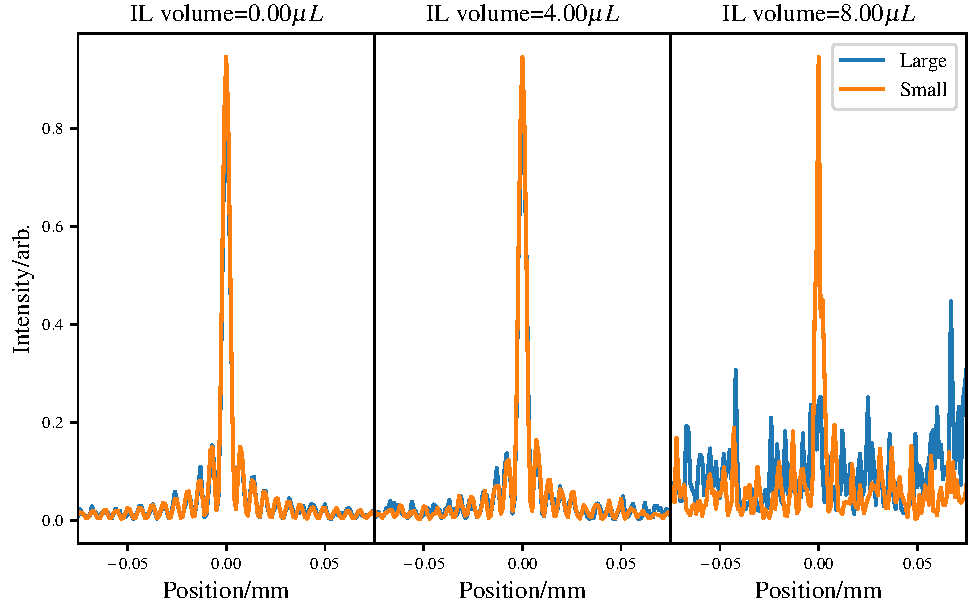
\includegraphics[width=0.7\textwidth]{compare-med-size.pdf}
    \caption{Comparison of a larger medium, $2~mm^3$ versus that of a smaller medium, $0.5~mm \times 0.5~mm \time 2.00~mm$.}
    \label{fig:compareBigSmall}
\end{figure}

\FloatBarrier

\section{Gaussian Beams}


\begin{equation}
E(r,z)=E_0\frac{w_0}{w(z)}e^{\frac{-r^2}{w(z)^2}}e^{-i(kz+k\frac{r^2}{2R(z)}-\varphi(z))}
\label{eqn:gaussefield}
\end{equation}

\noindent Where:

    \indent $r$ is the radial distance from the optical axis [$m$];

    \indent $z$ is the axial distance from  the beams waist [$m$];

    \indent $k$ is the wavenumber, $k=\frac{2\pi}{\lambda}$ [$m^{-1}$];

    \indent $E_0$ is the electric field amplitude at the origin [$Vm^{-1}$];

    \indent $w(z)$ is the radius of the beam at which the amplitude has fallen to $\frac{1}{e}$, at the distance z along the beam [$m$];

    \indent $w_0$ is the waist radius [$m$];

    \indent $R(z)$ is the radius of curvature of the beams wavefronts at z [$m$];

    \indent and finally, $\varphi(z)$ is the Gouy phase at z [-].


\begin{equation}
    w(z)= w_0\sqrt{1+\left(\frac{z}{z_r}\right)^2}
\label{eqn:gwaist}
\end{equation}
    
\begin{equation}
R(z)=z\left[1+\left(\frac{z_r}{z}\right)^2\right]
\label{eqn:radiuscurve}
\end{equation}

\begin{equation}
\varphi(z)=arctan\left(\frac{z}{z_r}\right)
\label{eqn:gouyphase}
\end{equation}

\begin{equation}
z_r = \frac{\pi w_0^2}{\lambda}
\label{eqn:rayleighrange}
\end{equation}

\begin{equation}
w_0=\frac{2\lambda f}{\pi D}
\label{eqn:beamwiast}
\end{equation}

\begin{figure}[!ht]
    \centering
    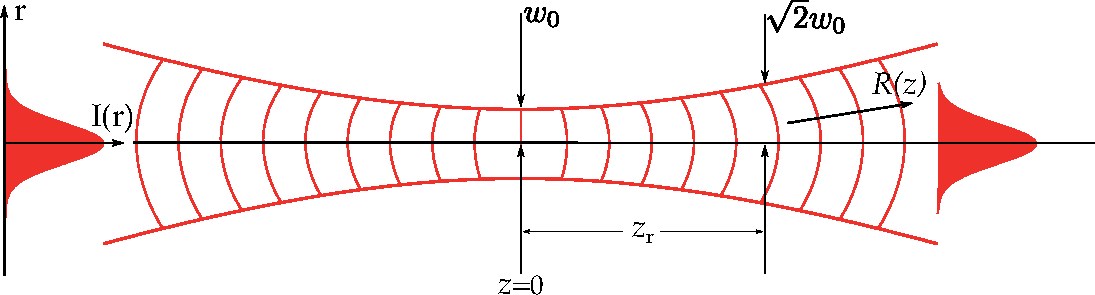
\includegraphics[width=0.95\textwidth]{gaussian-radius-curve.pdf}
    \caption{Illustration of a Gaussian beam focusing to its waist then diverging away. Image shows the various defined properties of a Gaussian beam along side the radius of curvature changing direction at the waist.}
    \label{fig:gbeamills}
\end{figure}


    


% gaussian beam theory
% geometry
% implementation of lens's -> plano-convex and aspheric
% emphasis no coding of focal distance
% spherical aberrations 
% curvature of phase change


\section{Higher order Bessel beams}

Our technique outlined in the preceding sections, can also be applied to arbitrary higher order Bessel beams. 

%why higher order useful

The electric field of a Bessel beam is:

\begin{equation}
E(r,\varphi,z)=E_0J_l(k_r r)e^{-i k_z z}e^{-i l \varphi}
\end{equation}

\noindent Where:

\indent l is the order of the beam [-];

\indent $k_{z}^{2} + k_{r}^{2} =k^2$, where $k^2$ is the wavevector [$m^{-1}$];

\indent $r, \varphi, and z$ are the cylindrical coordinates [$m$, $rad$, $m$];

\indent and $J_l$ is the l-order Bessel function of the first kind [-].

\medskip

%properties of higher order bssel beams

%methods of generating higher orders
To generate higher order Bessel beam, a helicon is used.
A helicon (shown in~\cref{fig:helix-2}) is an axicon attached to a helix phase delay element.
The helical element imparts a helical phase delay to photon packets as they pass through the element.


The distance travelled though the helicon is shown in~\cref{eqn:helix,eqn:axicon,eqn:heightdiff}\cite{wei2015generation}.
$h_1$ is the path length travelled by a photon through the helical element.
$h_2$ is the path through an axicon.

\begin{align}
h_1&=\frac{l\varphi\lambda}{(n-1)2\pi} \label{eqn:helix}\\
h_2&=r\ tan(\alpha)\label{eqn:axicon}\\
h_3&=h_1+h_2 \label{eqn:helicon}\\
\Delta h &= \frac{l\lambda}{n-1}\label{eqn:heightdiff}
\end{align}

Where $\varphi$ is the azimuthal angle, $r$ is the radial position, $l$ is  blah, and $\alpha$ is the axicon angle.

The path length in the above equations can be converted into a phase delay by considering the transmission functions of the individual elements~\cite{khonina1992trochoson,kotlyar2006diffraction,topuzoski2009conversion,qiong2012generalization}:


\begin{align}
T_1(\varphi)&=e^{-ik(n-1)h_1}=e^{-il\varphi}\\
T_2(r)&=e^{-ik(n-1)h_2}=e^{-ik_rr}\\
T_3(r,\varphi)&=T_1*T_2=e^{-ik_rr-il\varphi}\\
\end{align}

Where $T_1$ is the transmission function for the helical element, $T_2$ is the transmission function for the axicon, and $T_3$ is the total transmission function.
Using the small angle approximation  for $\beta$ and~\cref{eqn:betaangle}, and knowing $k_r=sin\left(\beta\right)$ yields the phase delay as a function of angle and radial position:

\begin{equation}
\phi(\varphi,r)=k(n-1)r\alpha+l\varphi
\end{equation}

To implement a helicon in the $\varphi MC$ algorithm, an additional helical phase delay is added.
The additional delay is implemented by adding $l\varphi$ where $0<varphi<\tfrac{2\pi}{l}$.
An actual helix element is not modelled explicitly in the code, but rather just the phase delay.
This method is similar to using a spatial light modulator in an experiment to impart a phase delay on a beam.

\Cref{fig:highordershow} shows the comparison between theoretical higher order Bessel beam and the higher order beam beam simulated by $\varphi MC$.

\begin{figure}[!ht]
    \centering
    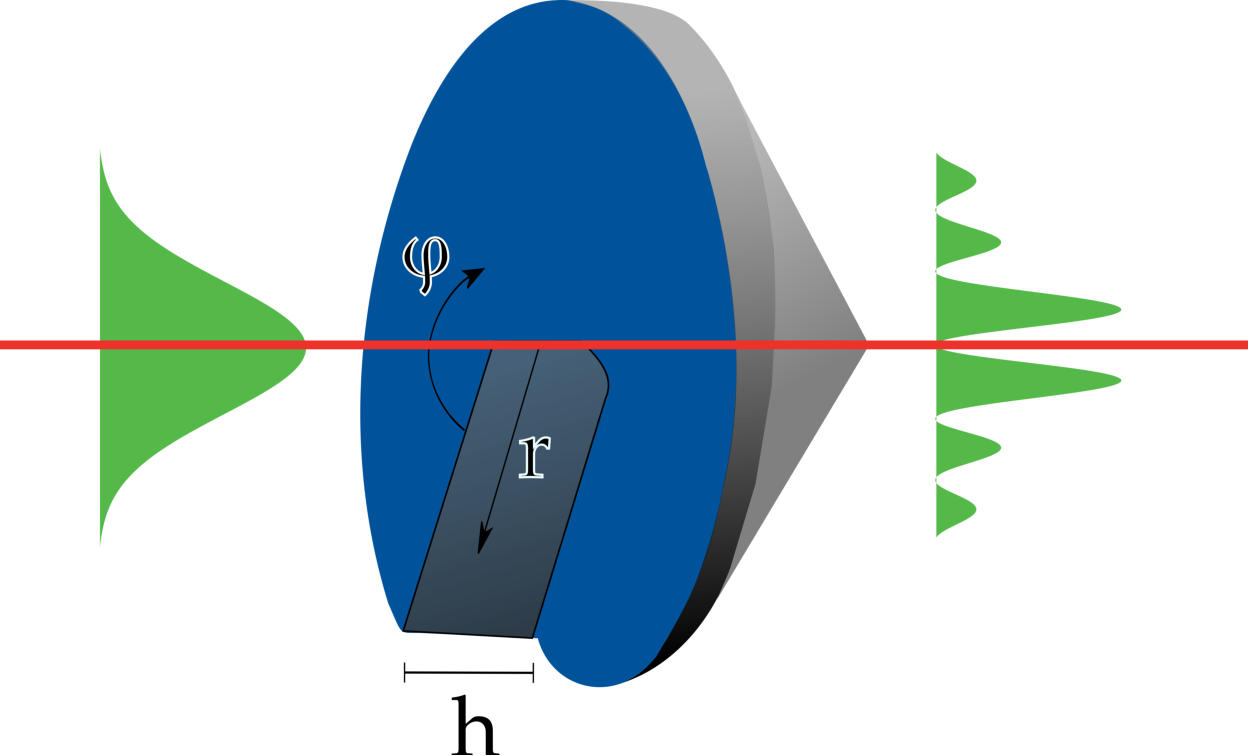
\includegraphics[width=0.4\textwidth]{helicon-2.pdf}
    \caption{Helical delay element attached to an axicon. Axicon introduces an additional radial delay in addition to that of the helical element. Input beam is a Gaussian, output beam is a higher order Bessel beam, $l>0$.}
    \label{fig:helix-2}
    \vspace{-10pt}
\end{figure}

\begin{figure}[!ht]
    \centering
    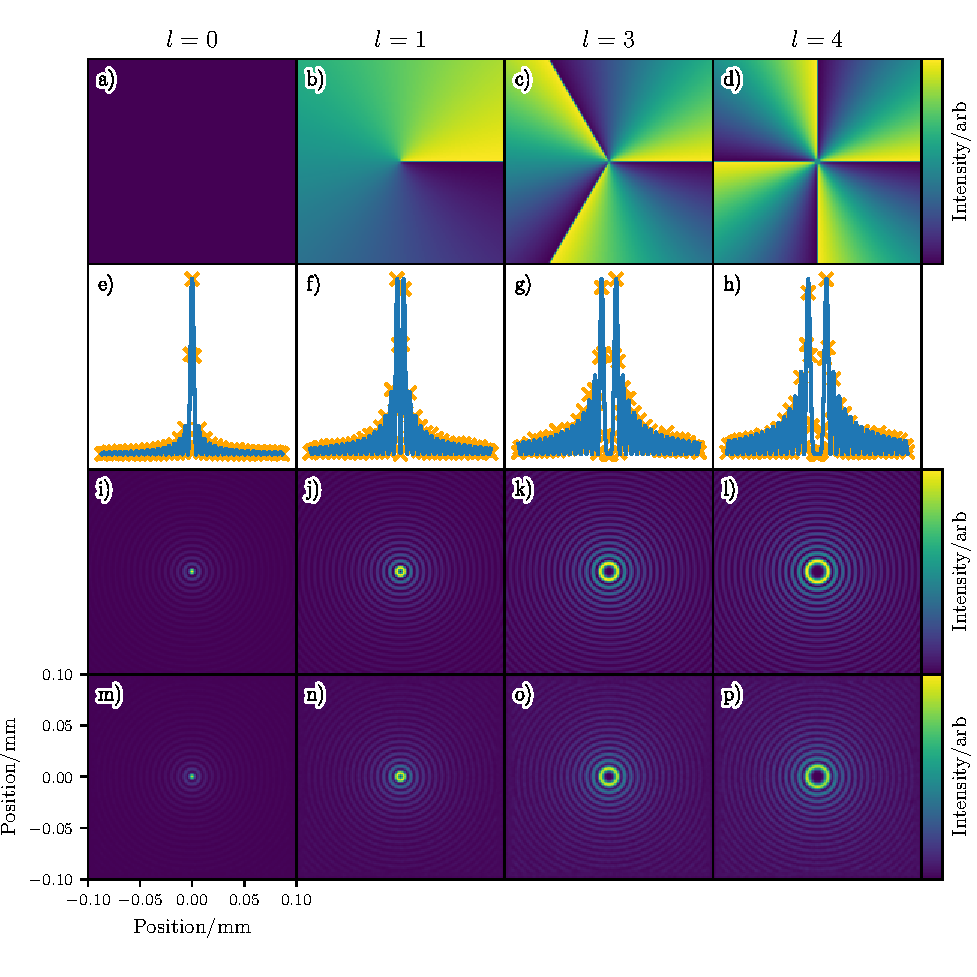
\includegraphics[width=0.85\textwidth]{higher-order-bessel.pdf}
    \caption{Higher order Bessel beams. a) to d) show the phase shift due to the helical element. e) to h) show line plots of the simulation data compared to the theory. i) to l) and m) to p) show the higher order Bessel beam images for theory and simulation data respectively.}
    \label{fig:highordershow}
\end{figure}

\FloatBarrier
\section{Comparison}

\section{Discussion}

%talk about comparison of beams. methods validity -> downside and upsides

a~\cite{mignon2016fractional}
\section{Conclusion}

%conclude shit


%sources
%cizmar thesis
%born: principles of optics
%hecht: optics
%mignon
%prahl
%fresnel/fraunhoefer paper
%thorlabs
%sacsha thesis
%kishans papers
%various axicon papers
%aspheric papers
%phase screen model
%beam steering paper
%paper that hates on mcrt
%E-field mcrt